\section{Virtual Memory}

From previous courses we know MMUs, TLBs and basic paged virtual memory operations. The uses for address translation include: Process Isolation, Shared Code Segments, Dynamic Memory Allocation and many more.


\subsection{Segments}

Before paging, there were segments. Before segments there where base and limit registers. These contained two addresses $B$ and $L$. A CPU access to an address $a$ is permitted iff $B \leq a < L$. Relocation registers are an enhanced form of base register. All CPU accesses are relocated by adding the offset: a CPU access to an address $a$ is translated to $B + a$. This allows each program to be compiled to run at the same address (e.g. 0x0000). \medskip
\begin{center}
	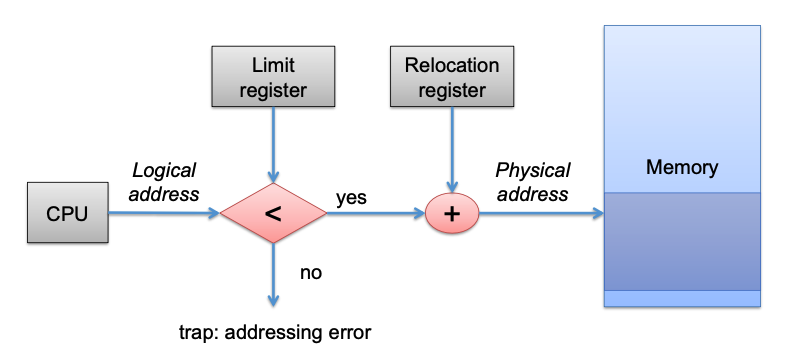
\includegraphics[width=\linewidth]{base-relocation-register.png}
\end{center}

A segment is a triple $(I, B_I, L_I)$ of values specifying a contiguous region of memory address space with base $B_I$, limit $L_I$, and an associated segment identifier $I$ which names the segment. Memory in a segmented system uses a form of logical addressing: each address is a pair $(I, O)$ of segment identifier and offset. A Segment Table is an in-memory array of base and limit values $(B_I, L_I)$ indexed by segment identifier, and possibly with additional protection information.
\begin{center}
	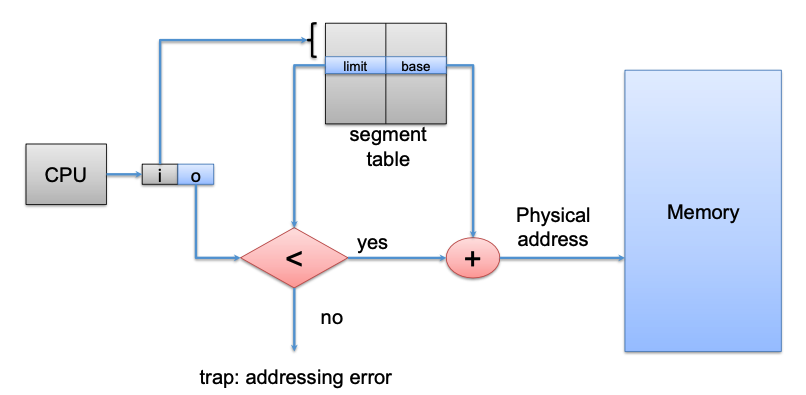
\includegraphics[width=\linewidth]{segment.png}
\end{center}

This enables sharing code/data segments between processes, further it adds protection and allows transparently growing stack/heap as needed. The principal downside of segmentation is that segments are still contiguous in physical memory, which leads to external fragmentation.


\subsection{Paging}

This is a short recap of paging. Virtual memory is divided into (virtual) pages of the same size having a VPN, physical memory gets divided into frames / physical pages having a PFN / PPN. Then a page table gets used to map VPNs to PFNs. This is implemented in hardware as the MMU. To speed up translation the TLB is used. Getting data from memory can work as follows (in this case we have a TLB miss):
\begin{center}
	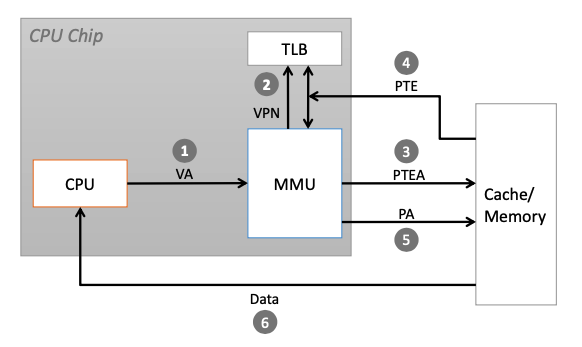
\includegraphics[width=\linewidth]{tlb-miss.png}
\end{center}

We have also seen how multi-level page tables work. Multi-level translation allows us to allocate only page table entries that are in use and makes memory allocation simpler.
\begin{center}
	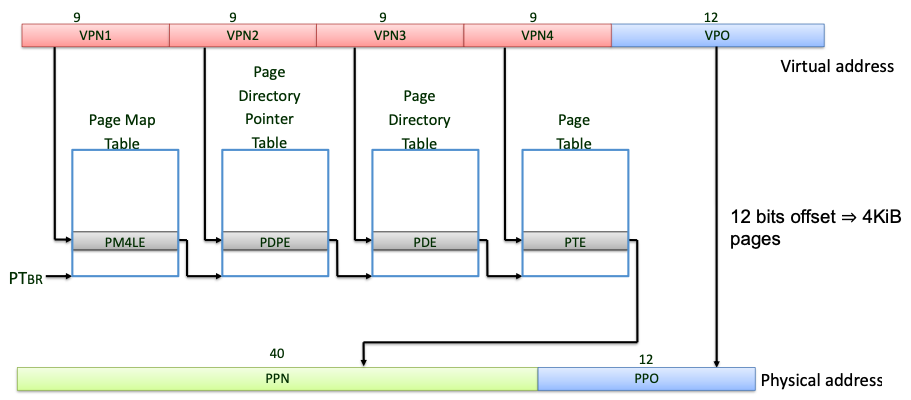
\includegraphics[width=\linewidth]{multi-level-pt.png}
\end{center}

On a context switch we need to store/restore the pointer to the page table and its size. One of the downsides of paging is if our page is very small and we do not need all of the space, this leads to internal fragmentation.


\subsection{Paged Segmentation}

It is possible to combine segmentation and paging. A paged segmentation memory management scheme is one where memory is addressed by a pair (segment.id, offset), as in a segmentation scheme, but each segment is itself composed of fixed-size pages whose page numbers are then translated to physical page numbers by a paged MMU.
\begin{center}
	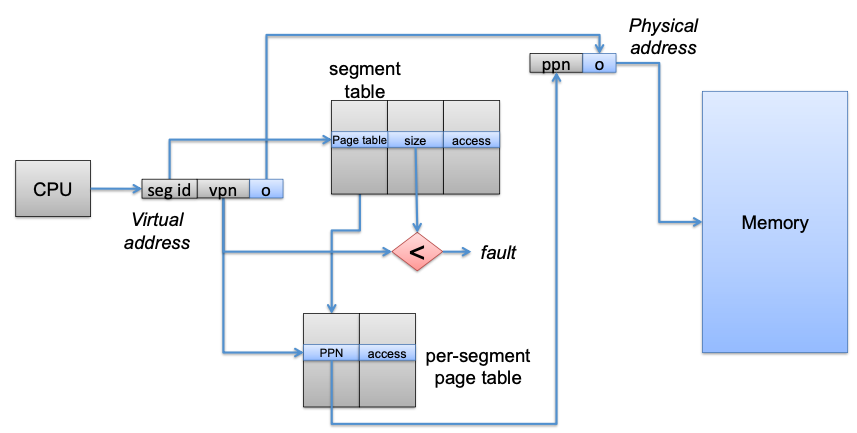
\includegraphics[width=\linewidth]{paged-segments.png}
\end{center}

One of the main benefits here is that each segment can have its own size of page table.


\subsection{Zero-on Reference}

The question how much physical memory is needed, is difficult to answer. So when a program runs out of memory, the system does the following:
\begin{enumerate}
	\item Page fault into OS kernel
	\item Kernel allocates some memory
	\item Zeroes the memory
	\item Modify page table
	\item Resume process
\end{enumerate}


\subsection{Fill On Demand}

Most programs do not need all their code to start running and might never use some code in its execution. Therefore we want to do something similar, we want to start a program before its code is in physical memory:
\begin{enumerate}
	\item Set all page table entries to invalid
	\item On first page reference, kernel trap
	\item Kernel brings page in from disk
	\item Resume execution
	\item Remaining pages can be transferred in the background while the program is running
\end{enumerate}


\subsection{Copy On Write}

Remember that we said \textit{fork()} copies the entire address space. This can be expensive and might not feasible in performance. On \textit{fork()} we copy the page table and set all mappings to read-only in both address spaces. Reads are now possible for both processes. If a write in either process causes a protection fault the kernel allocates a new frame and copies the referenced frames content into it. The faulting process now maps to the new copy and the protection changes to read/write (also for the non-faulting process).


\subsection{Managing Caches and the TLB}

\subsubsection{TLBs}

A problem with TLBs on context switches is that they can hold content inaccessible to the new process. To avoid having to flush the TLB, we introduce tags. Each TLB entry has a $6$-bit tag and the OS keeps track of a mapping between processes and tags. \medskip

\subsubsection{Caches}

\begin{center}
	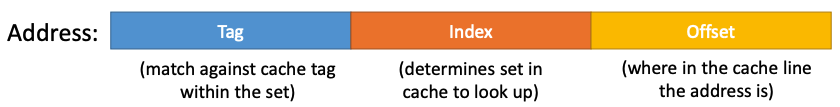
\includegraphics[width=\linewidth]{address.png}
\end{center}

Remember the different types of caches:
\begin{itemize}
	\item Virtually indexed, virtually tagged - simple and fast, but context switches are hard
	\item Physically indexed, physically tagged - can only be accessed after address translation
	\item Virtually indexed, physically tagged - overlap cache and TLB lookups
	\item Physically indexed, virtually tagged
\end{itemize}

Also remember the different write (write through, write back) and allocate (write allocate, non-write allocate) policies. In virtually tagged caches we can encounter homonyms, the same virtual address maps to multiple physical address spaces. To avoid this we can use physical tags, add address space identifiers, try to ensure disjoint address spaces or flush the cache on a context switch. \medskip

There is also a synonyms problem, where two virtual addresses map to the same physical address. This leads to inconsistent cache entries. The solutions to the homonym problem do not help here. To solve this problem we restrict VM mappings, so that synonyms map to the same cache set. 


\subsection{Demand Paging}

Demand paging solves the problem how to find a frame to use for missing pages. The goal is to minimize the page fault rate $p$ ($0 \leq p \leq 1$). The metric we are interested in is the effective access time $(1-p) * l_m + p * l_f$, where $l_m$ is the latency of a memory access and $l_p$ the latency of a page fault handling. Generally speaking the performance of a paging system depends on how many frames it has, but there is a diminishing return on adding new frames.

\subsubsection{Page Replacement Policies}

If a page has to be evicted, which one should be choose? We have already seen Least Recently Used (LRU) and First In First Out (FIFO). Both of these are not optimal, LRU is too expensive and FIFA works poorly for most workloads. A good compromise is the \textbf{Clock} or \textbf{2nd Chance} algorithm. It approximates LRU but much cheaper. It requires a linear table of all PFNs, with associated referenced bits. This can be best visualized as a circular buffer.
\begin{center}
	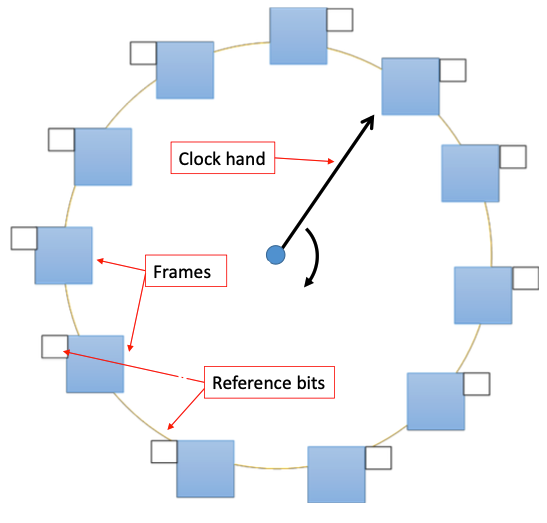
\includegraphics[width=0.8\linewidth]{2nd.png}
\end{center}

It works as follows:
\begin{itemize}
	\item Mark each frame when referenced for the first time
	\item If we want to replace a frame, process as follows: 
		\begin{itemize}
			\item If marked, unmark and advance the clock hand
			\item If unmarked, allocate this frame and mark it
		\end{itemize}
\end{itemize}

\subsubsection{Frame States}

\begin{center}
	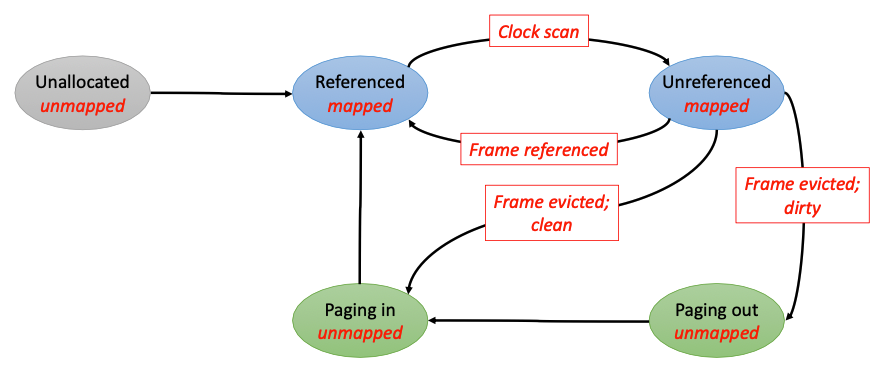
\includegraphics[width=\linewidth]{state_machine.png}
\end{center}

This only works if the corresponding bits are present in the page table and are properly set, in RISC-V for example these bits are present but do not have to be set. We can emulate these bits using faults.
